\documentclass[1p]{elsarticle_modified}
%\bibliographystyle{elsarticle-num}

%\usepackage[colorlinks]{hyperref}
%\usepackage{abbrmath_seonhwa} %\Abb, \Ascr, \Acal ,\Abf, \Afrak
\usepackage{amsfonts}
\usepackage{amssymb}
\usepackage{amsmath}
\usepackage{amsthm}
\usepackage{scalefnt}
\usepackage{amsbsy}
\usepackage{kotex}
\usepackage{caption}
\usepackage{subfig}
\usepackage{color}
\usepackage{graphicx}
\usepackage{xcolor} %% white, black, red, green, blue, cyan, magenta, yellow
\usepackage{float}
\usepackage{setspace}
\usepackage{hyperref}

\usepackage{tikz}
\usetikzlibrary{arrows}

\usepackage{multirow}
\usepackage{array} % fixed length table
\usepackage{hhline}

%%%%%%%%%%%%%%%%%%%%%
\makeatletter
\renewcommand*\env@matrix[1][\arraystretch]{%
	\edef\arraystretch{#1}%
	\hskip -\arraycolsep
	\let\@ifnextchar\new@ifnextchar
	\array{*\c@MaxMatrixCols c}}
\makeatother %https://tex.stackexchange.com/questions/14071/how-can-i-increase-the-line-spacing-in-a-matrix
%%%%%%%%%%%%%%%

\usepackage[normalem]{ulem}

\newcommand{\msout}[1]{\ifmmode\text{\sout{\ensuremath{#1}}}\else\sout{#1}\fi}
%SOURCE: \msout is \stkout macro in https://tex.stackexchange.com/questions/20609/strikeout-in-math-mode

\newcommand{\cancel}[1]{
	\ifmmode
	{\color{red}\msout{#1}}
	\else
	{\color{red}\sout{#1}}
	\fi
}

\newcommand{\add}[1]{
	{\color{blue}\uwave{#1}}
}

\newcommand{\replace}[2]{
	\ifmmode
	{\color{red}\msout{#1}}{\color{blue}\uwave{#2}}
	\else
	{\color{red}\sout{#1}}{\color{blue}\uwave{#2}}
	\fi
}

\newcommand{\Sol}{\mathcal{S}} %segment
\newcommand{\D}{D} %diagram
\newcommand{\A}{\mathcal{A}} %arc


%%%%%%%%%%%%%%%%%%%%%%%%%%%%%5 test

\def\sl{\operatorname{\textup{SL}}(2,\Cbb)}
\def\psl{\operatorname{\textup{PSL}}(2,\Cbb)}
\def\quan{\mkern 1mu \triangleright \mkern 1mu}

\theoremstyle{definition}
\newtheorem{thm}{Theorem}[section]
\newtheorem{prop}[thm]{Proposition}
\newtheorem{lem}[thm]{Lemma}
\newtheorem{ques}[thm]{Question}
\newtheorem{cor}[thm]{Corollary}
\newtheorem{defn}[thm]{Definition}
\newtheorem{exam}[thm]{Example}
\newtheorem{rmk}[thm]{Remark}
\newtheorem{alg}[thm]{Algorithm}

\newcommand{\I}{\sqrt{-1}}
\begin{document}

%\begin{frontmatter}
%
%\title{Boundary parabolic representations of knots up to 8 crossings}
%
%%% Group authors per affiliation:
%\author{Yunhi Cho} 
%\address{Department of Mathematics, University of Seoul, Seoul, Korea}
%\ead{yhcho@uos.ac.kr}
%
%
%\author{Seonhwa Kim} %\fnref{s_kim}}
%\address{Center for Geometry and Physics, Institute for Basic Science, Pohang, 37673, Korea}
%\ead{ryeona17@ibs.re.kr}
%
%\author{Hyuk Kim}
%\address{Department of Mathematical Sciences, Seoul National University, Seoul 08826, Korea}
%\ead{hyukkim@snu.ac.kr}
%
%\author{Seokbeom Yoon}
%\address{Department of Mathematical Sciences, Seoul National University, Seoul, 08826,  Korea}
%\ead{sbyoon15@snu.ac.kr}
%
%\begin{abstract}
%We find all boundary parabolic representation of knots up to 8 crossings.
%
%\end{abstract}
%\begin{keyword}
%    \MSC[2010] 57M25 
%\end{keyword}
%
%\end{frontmatter}

%\linenumbers
%\tableofcontents
%
\newcommand\colored[1]{\textcolor{white}{\rule[-0.35ex]{0.8em}{1.4ex}}\kern-0.8em\color{red} #1}%
%\newcommand\colored[1]{\textcolor{white}{ #1}\kern-2.17ex	\textcolor{white}{ #1}\kern-1.81ex	\textcolor{white}{ #1}\kern-2.15ex\color{red}#1	}

{\Large $\underline{11n_{111}~(K11n_{111})}$}

\setlength{\tabcolsep}{10pt}
\renewcommand{\arraystretch}{1.6}
\vspace{1cm}\begin{tabular}{m{100pt}>{\centering\arraybackslash}m{274pt}}
\multirow{5}{120pt}{
	\centering
	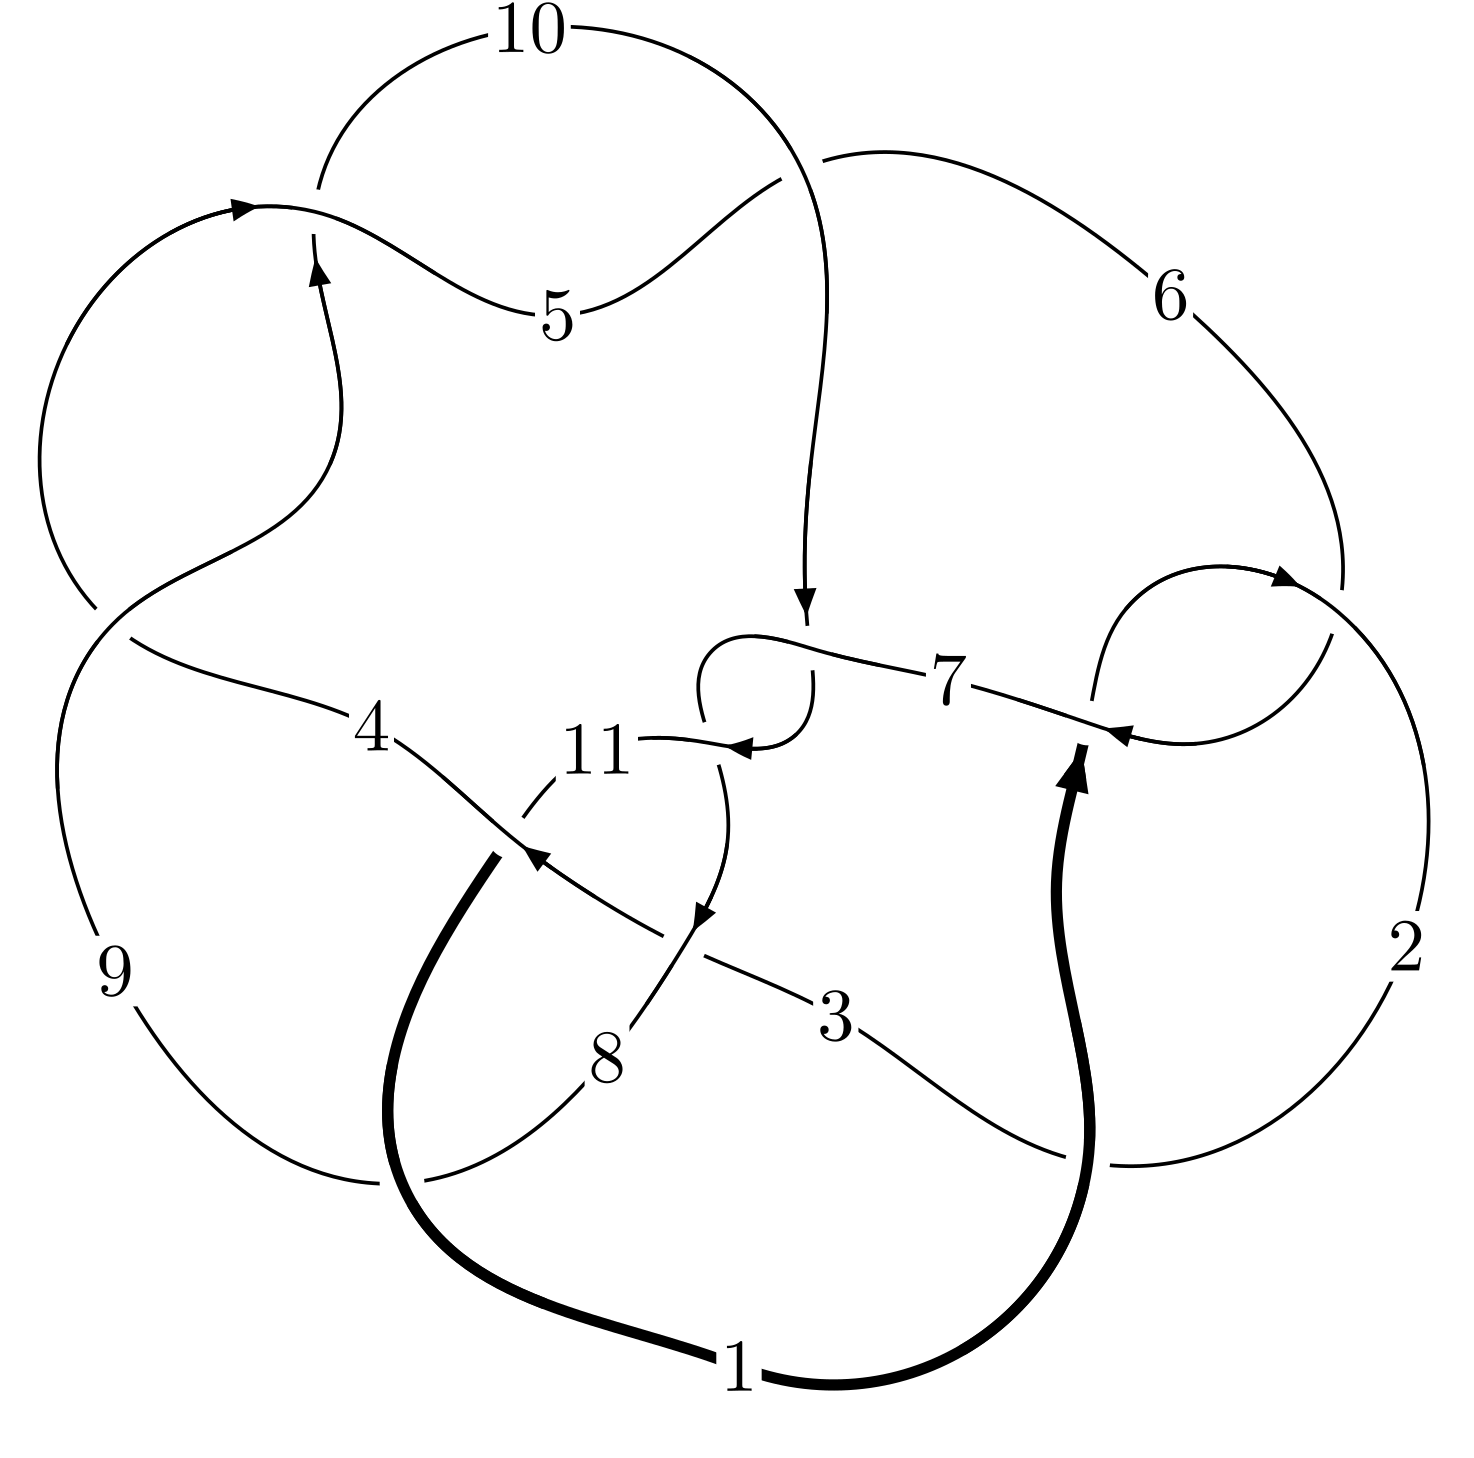
\includegraphics[width=112pt]{../../../GIT/diagram.site/Diagrams/png/727_11n_111.png}\\
\ \ \ A knot diagram\footnotemark}&
\allowdisplaybreaks
\textbf{Linearized knot diagam} \\
\cline{2-2}
 &
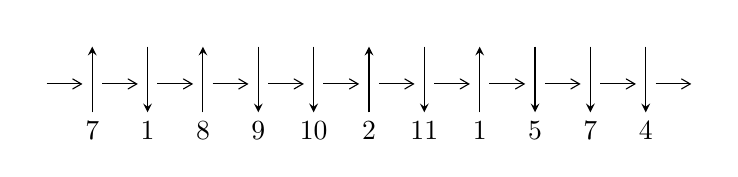
\begin{tikzpicture}[x=20pt, y=17pt]
	% nodes
	\node (C0) at (0, 0) {};
	\node (C1) at (1, 0) {};
	\node (C1U) at (1, +1) {};
	\node (C1D) at (1, -1) {7};

	\node (C2) at (2, 0) {};
	\node (C2U) at (2, +1) {};
	\node (C2D) at (2, -1) {1};

	\node (C3) at (3, 0) {};
	\node (C3U) at (3, +1) {};
	\node (C3D) at (3, -1) {8};

	\node (C4) at (4, 0) {};
	\node (C4U) at (4, +1) {};
	\node (C4D) at (4, -1) {9};

	\node (C5) at (5, 0) {};
	\node (C5U) at (5, +1) {};
	\node (C5D) at (5, -1) {10};

	\node (C6) at (6, 0) {};
	\node (C6U) at (6, +1) {};
	\node (C6D) at (6, -1) {2};

	\node (C7) at (7, 0) {};
	\node (C7U) at (7, +1) {};
	\node (C7D) at (7, -1) {11};

	\node (C8) at (8, 0) {};
	\node (C8U) at (8, +1) {};
	\node (C8D) at (8, -1) {1};

	\node (C9) at (9, 0) {};
	\node (C9U) at (9, +1) {};
	\node (C9D) at (9, -1) {5};

	\node (C10) at (10, 0) {};
	\node (C10U) at (10, +1) {};
	\node (C10D) at (10, -1) {7};

	\node (C11) at (11, 0) {};
	\node (C11U) at (11, +1) {};
	\node (C11D) at (11, -1) {4};
	\node (C12) at (12, 0) {};

	% arrows
	\draw[->,>={angle 60}]
	(C0) edge (C1) (C1) edge (C2) (C2) edge (C3) (C3) edge (C4) (C4) edge (C5) (C5) edge (C6) (C6) edge (C7) (C7) edge (C8) (C8) edge (C9) (C9) edge (C10) (C10) edge (C11) (C11) edge (C12) ;	\draw[->,>=stealth]
	(C1D) edge (C1U) (C2U) edge (C2D) (C3D) edge (C3U) (C4U) edge (C4D) (C5U) edge (C5D) (C6D) edge (C6U) (C7U) edge (C7D) (C8D) edge (C8U) (C9U) edge (C9D) (C10U) edge (C10D) (C11U) edge (C11D) ;
	\end{tikzpicture} \\
\hhline{~~} \\& 
\textbf{Solving Sequence} \\ \cline{2-2} 
 &
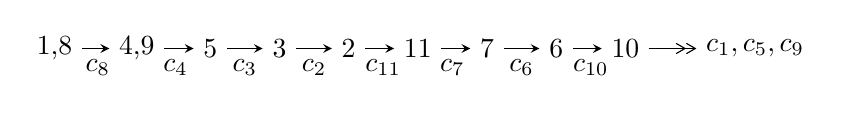
\begin{tikzpicture}[x=25pt, y=7pt]
	% node
	\node (A0) at (-1/8, 0) {1,8};
	\node (A1) at (17/16, 0) {4,9};
	\node (A2) at (17/8, 0) {5};
	\node (A3) at (25/8, 0) {3};
	\node (A4) at (33/8, 0) {2};
	\node (A5) at (41/8, 0) {11};
	\node (A6) at (49/8, 0) {7};
	\node (A7) at (57/8, 0) {6};
	\node (A8) at (65/8, 0) {10};
	\node (C1) at (1/2, -1) {$c_{8}$};
	\node (C2) at (13/8, -1) {$c_{4}$};
	\node (C3) at (21/8, -1) {$c_{3}$};
	\node (C4) at (29/8, -1) {$c_{2}$};
	\node (C5) at (37/8, -1) {$c_{11}$};
	\node (C6) at (45/8, -1) {$c_{7}$};
	\node (C7) at (53/8, -1) {$c_{6}$};
	\node (C8) at (61/8, -1) {$c_{10}$};
	\node (A9) at (10, 0) {$c_{1},c_{5},c_{9}$};

	% edge
	\draw[->,>=stealth]	
	(A0) edge (A1) (A1) edge (A2) (A2) edge (A3) (A3) edge (A4) (A4) edge (A5) (A5) edge (A6) (A6) edge (A7) (A7) edge (A8) ;
	\draw[->>,>={angle 60}]	
	(A8) edge (A9);
\end{tikzpicture} \\ 

\end{tabular} \\

\footnotetext{
The image of knot diagram is generated by the software ``\textbf{Draw programme}" developed by Andrew Bartholomew(\url{http://www.layer8.co.uk/maths/draw/index.htm\#Running-draw}), where we modified some parts for our purpose(\url{https://github.com/CATsTAILs/LinksPainter}).
}\phantom \\ \newline 
\centering \textbf{Ideals for irreducible components\footnotemark of $X_{\text{par}}$} 
 
\begin{align*}
I^u_{1}&=\langle 
-249708 u^9-1442317 u^8+\cdots+48083962 b-1389936,\\
\phantom{I^u_{1}}&\phantom{= \langle  }2808285 u^9-11413026 u^8+\cdots+625091506 a-1233253,\\
\phantom{I^u_{1}}&\phantom{= \langle  }u^{10}+u^9-3 u^8-11 u^7+23 u^6+10 u^5-40 u^4+43 u^3+8 u-13\rangle \\
I^u_{2}&=\langle 
-9 u^6+10 u^5-29 u^4-13 u^3+37 u^2+41 b-95 u+37,\\
\phantom{I^u_{2}}&\phantom{= \langle  }-7 u^6+26 u^5-18 u^4+40 u^3+88 u^2+41 a-124 u+129,\;u^7+3 u^5+3 u^4-2 u^3+7 u^2-2 u+1\rangle \\
\\
\end{align*}
\raggedright * 2 irreducible components of $\dim_{\mathbb{C}}=0$, with total 17 representations.\\
\footnotetext{All coefficients of polynomials are rational numbers. But the coefficients are sometimes approximated in decimal forms when there is not enough margin.}
\newpage
\renewcommand{\arraystretch}{1}
\centering \section*{I. $I^u_{1}= \langle -2.50\times10^{5} u^{9}-1.44\times10^{6} u^{8}+\cdots+4.81\times10^{7} b-1.39\times10^{6},\;2.81\times10^{6} u^{9}-1.14\times10^{7} u^{8}+\cdots+6.25\times10^{8} a-1.23\times10^{6},\;u^{10}+u^9+\cdots+8 u-13 \rangle$}
\flushleft \textbf{(i) Arc colorings}\\
\begin{tabular}{m{7pt} m{180pt} m{7pt} m{180pt} }
\flushright $a_{1}=$&$\begin{pmatrix}0\\u\end{pmatrix}$ \\
\flushright $a_{8}=$&$\begin{pmatrix}1\\0\end{pmatrix}$ \\
\flushright $a_{4}=$&$\begin{pmatrix}-0.00449260 u^{9}+0.0182582 u^{8}+\cdots+1.32084 u+0.00197292\\0.00519317 u^{9}+0.0299958 u^{8}+\cdots+0.743464 u+0.0289064\end{pmatrix}$ \\
\flushright $a_{9}=$&$\begin{pmatrix}1\\- u^2\end{pmatrix}$ \\
\flushright $a_{5}=$&$\begin{pmatrix}-0.0220573 u^{9}-0.0351316 u^{8}+\cdots+0.817782 u-0.322693\\0.0438996 u^{9}+0.0820347 u^{8}+\cdots+0.685204 u+0.494633\end{pmatrix}$ \\
\flushright $a_{3}=$&$\begin{pmatrix}-0.00968576 u^{9}-0.0117376 u^{8}+\cdots+0.577372 u-0.0269335\\0.00519317 u^{9}+0.0299958 u^{8}+\cdots+0.743464 u+0.0289064\end{pmatrix}$ \\
\flushright $a_{2}=$&$\begin{pmatrix}-0.00968576 u^{9}-0.0117376 u^{8}+\cdots+0.577372 u-0.0269335\\0.0214765 u^{9}+0.0741603 u^{8}+\cdots+0.852964 u+0.0555807\end{pmatrix}$ \\
\flushright $a_{11}=$&$\begin{pmatrix}0.0198337 u^{9}+0.0277149 u^{8}+\cdots-0.545921 u+0.561441\\0.0210232 u^{9}+0.0419173 u^{8}+\cdots+0.718255 u+0.381521\end{pmatrix}$ \\
\flushright $a_{7}=$&$\begin{pmatrix}0.00222357 u^{9}+0.00741674 u^{8}+\cdots-0.271861 u+0.761252\\-0.0347357 u^{9}-0.0812062 u^{8}+\cdots-0.339580 u-0.451264\end{pmatrix}$ \\
\flushright $a_{6}=$&$\begin{pmatrix}0.0336232 u^{9}+0.0761229 u^{8}+\cdots-0.224398 u+0.840205\\-0.0855628 u^{9}-0.203256 u^{8}+\cdots-0.398771 u-1.06216\end{pmatrix}$ \\
\flushright $a_{10}=$&$\begin{pmatrix}0.0238374 u^{9}+0.0435082 u^{8}+\cdots-0.0666326 u+0.770268\\-0.00441748 u^{9}+0.00115972 u^{8}+\cdots+0.414900 u+0.184888\end{pmatrix}$\\ \flushright $a_{10}=$&$\begin{pmatrix}0.0238374 u^{9}+0.0435082 u^{8}+\cdots-0.0666326 u+0.770268\\-0.00441748 u^{9}+0.00115972 u^{8}+\cdots+0.414900 u+0.184888\end{pmatrix}$\\&\end{tabular}
\flushleft \textbf{(ii) Obstruction class $= -1$}\\~\\
\flushleft \textbf{(iii) Cusp Shapes $= -\frac{5126407}{48083962} u^9-\frac{1515297}{48083962} u^8+\cdots+\frac{151141541}{48083962} u-\frac{241733105}{48083962}$}\\~\\
\newpage\renewcommand{\arraystretch}{1}
\flushleft \textbf{(iv) u-Polynomials at the component}\newline \\
\begin{tabular}{m{50pt}|m{274pt}}
Crossings & \hspace{64pt}u-Polynomials at each crossing \\
\hline $$\begin{aligned}c_{1},c_{3},c_{6}\end{aligned}$$&$\begin{aligned}
&u^{10}-6 u^8-4 u^7+31 u^6-3 u^5+19 u^4-2 u^3+u^2+u-1
\end{aligned}$\\
\hline $$\begin{aligned}c_{2}\end{aligned}$$&$\begin{aligned}
&u^{10}-12 u^9+\cdots-3 u+1
\end{aligned}$\\
\hline $$\begin{aligned}c_{4},c_{5},c_{9}\end{aligned}$$&$\begin{aligned}
&u^{10}-9 u^9+36 u^8-79 u^7+93 u^6-36 u^5-40 u^4+45 u^3-8 u^2+4 u-8
\end{aligned}$\\
\hline $$\begin{aligned}c_{7},c_{10}\end{aligned}$$&$\begin{aligned}
&u^{10}+3 u^9+11 u^8+u^7-9 u^6-84 u^5-64 u^4-11 u^3-16 u^2-1
\end{aligned}$\\
\hline $$\begin{aligned}c_{8}\end{aligned}$$&$\begin{aligned}
&u^{10}- u^9-3 u^8+11 u^7+23 u^6-10 u^5-40 u^4-43 u^3-8 u-13
\end{aligned}$\\
\hline $$\begin{aligned}c_{11}\end{aligned}$$&$\begin{aligned}
&u^{10}-2 u^9+u^8+2 u^7+u^6-7 u^5+7 u^4- u^2-2 u+1
\end{aligned}$\\
\hline
\end{tabular}\\~\\
\newpage\renewcommand{\arraystretch}{1}
\flushleft \textbf{(v) Riley Polynomials at the component}\newline \\
\begin{tabular}{m{50pt}|m{274pt}}
Crossings & \hspace{64pt}Riley Polynomials at each crossing \\
\hline $$\begin{aligned}c_{1},c_{3},c_{6}\end{aligned}$$&$\begin{aligned}
&y^{10}-12 y^9+\cdots-3 y+1
\end{aligned}$\\
\hline $$\begin{aligned}c_{2}\end{aligned}$$&$\begin{aligned}
&y^{10}+52 y^9+\cdots-75 y+1
\end{aligned}$\\
\hline $$\begin{aligned}c_{4},c_{5},c_{9}\end{aligned}$$&$\begin{aligned}
&y^{10}-9 y^9+\cdots+112 y+64
\end{aligned}$\\
\hline $$\begin{aligned}c_{7},c_{10}\end{aligned}$$&$\begin{aligned}
&y^{10}+13 y^9+\cdots+32 y+1
\end{aligned}$\\
\hline $$\begin{aligned}c_{8}\end{aligned}$$&$\begin{aligned}
&y^{10}-7 y^9+\cdots-64 y+169
\end{aligned}$\\
\hline $$\begin{aligned}c_{11}\end{aligned}$$&$\begin{aligned}
&y^{10}-2 y^9+\cdots-6 y+1
\end{aligned}$\\
\hline
\end{tabular}\\~\\
\newpage\flushleft \textbf{(vi) Complex Volumes and Cusp Shapes}
$$\begin{array}{c|c|c}  
\text{Solutions to }I^u_{1}& \I (\text{vol} + \sqrt{-1}CS) & \text{Cusp shape}\\
 \hline 
\begin{aligned}
u &= \phantom{-}0.661040 + 0.972526 I \\
a &= \phantom{-}0.046863 + 1.141840 I \\
b &= \phantom{-}0.139003 + 0.708370 I\end{aligned}
 & -5.08678 + 3.48759 I & -7.45675 - 0.73295 I \\ \hline\begin{aligned}
u &= \phantom{-}0.661040 - 0.972526 I \\
a &= \phantom{-}0.046863 - 1.141840 I \\
b &= \phantom{-}0.139003 - 0.708370 I\end{aligned}
 & -5.08678 - 3.48759 I & -7.45675 + 0.73295 I \\ \hline\begin{aligned}
u &= \phantom{-}0.672063\phantom{ +0.000000I} \\
a &= \phantom{-}0.745125\phantom{ +0.000000I} \\
b &= \phantom{-}0.447351\phantom{ +0.000000I}\end{aligned}
 & -1.57143\phantom{ +0.000000I} & -5.48950\phantom{ +0.000000I} \\ \hline\begin{aligned}
u &= -0.334564 + 0.528443 I \\
a &= -0.220981 + 1.025590 I \\
b &= -0.178308 + 0.529060 I\end{aligned}
 & -0.164338 - 1.117660 I & -2.63384 + 5.74501 I \\ \hline\begin{aligned}
u &= -0.334564 - 0.528443 I \\
a &= -0.220981 - 1.025590 I \\
b &= -0.178308 - 0.529060 I\end{aligned}
 & -0.164338 + 1.117660 I & -2.63384 - 5.74501 I \\ \hline\begin{aligned}
u &= -1.57545\phantom{ +0.000000I} \\
a &= -0.500640\phantom{ +0.000000I} \\
b &= -0.399391\phantom{ +0.000000I}\end{aligned}
 & -10.0735\phantom{ +0.000000I} & -16.9190\phantom{ +0.000000I} \\ \hline\begin{aligned}
u &= \phantom{-}1.61793 + 0.67025 I \\
a &= \phantom{-}0.679052 + 0.329399 I \\
b &= -2.13328 - 0.91289 I\end{aligned}
 & \phantom{-}7.01395 + 1.69275 I & -4.50434 - 0.09697 I \\ \hline\begin{aligned}
u &= \phantom{-}1.61793 - 0.67025 I \\
a &= \phantom{-}0.679052 - 0.329399 I \\
b &= -2.13328 + 0.91289 I\end{aligned}
 & \phantom{-}7.01395 - 1.69275 I & -4.50434 + 0.09697 I \\ \hline\begin{aligned}
u &= -1.99271 + 1.85205 I \\
a &= -0.050253 - 0.499314 I \\
b &= \phantom{-}2.14860 - 1.33539 I\end{aligned}
 & \phantom{-}6.52702 - 8.61249 I & -5.20069 + 4.18606 I \\ \hline\begin{aligned}
u &= -1.99271 - 1.85205 I \\
a &= -0.050253 + 0.499314 I \\
b &= \phantom{-}2.14860 + 1.33539 I\end{aligned}
 & \phantom{-}6.52702 + 8.61249 I & -5.20069 - 4.18606 I\\
 \hline 
 \end{array}$$\newpage\newpage\renewcommand{\arraystretch}{1}
\centering \section*{II. $I^u_{2}= \langle -9 u^6+10 u^5+\cdots+41 b+37,\;-7 u^6+26 u^5+\cdots+41 a+129,\;u^7+3 u^5+3 u^4-2 u^3+7 u^2-2 u+1 \rangle$}
\flushleft \textbf{(i) Arc colorings}\\
\begin{tabular}{m{7pt} m{180pt} m{7pt} m{180pt} }
\flushright $a_{1}=$&$\begin{pmatrix}0\\u\end{pmatrix}$ \\
\flushright $a_{8}=$&$\begin{pmatrix}1\\0\end{pmatrix}$ \\
\flushright $a_{4}=$&$\begin{pmatrix}0.170732 u^{6}-0.634146 u^{5}+\cdots+3.02439 u-3.14634\\0.219512 u^{6}-0.243902 u^{5}+\cdots+2.31707 u-0.902439\end{pmatrix}$ \\
\flushright $a_{9}=$&$\begin{pmatrix}1\\- u^2\end{pmatrix}$ \\
\flushright $a_{5}=$&$\begin{pmatrix}0.0243902 u^{6}-0.804878 u^{5}+\cdots+2.14634 u-2.87805\\0.585366 u^{6}-0.317073 u^{5}+\cdots+2.51220 u-1.07317\end{pmatrix}$ \\
\flushright $a_{3}=$&$\begin{pmatrix}-0.0487805 u^{6}-0.390244 u^{5}+\cdots+0.707317 u-2.24390\\0.219512 u^{6}-0.243902 u^{5}+\cdots+2.31707 u-0.902439\end{pmatrix}$ \\
\flushright $a_{2}=$&$\begin{pmatrix}-0.0487805 u^{6}-0.390244 u^{5}+\cdots+0.707317 u-2.24390\\0.341463 u^{6}-0.268293 u^{5}+\cdots+3.04878 u-1.29268\end{pmatrix}$ \\
\flushright $a_{11}=$&$\begin{pmatrix}0.878049 u^{6}+1.02439 u^{5}+\cdots+3.26829 u+2.39024\\0.0487805 u^{6}+0.390244 u^{5}+\cdots+0.292683 u+1.24390\end{pmatrix}$ \\
\flushright $a_{7}=$&$\begin{pmatrix}-0.902439 u^{6}-0.219512 u^{5}+\cdots-5.41463 u-0.512195\\-0.390244 u^{6}-0.121951 u^{5}+\cdots-1.34146 u-0.951220\end{pmatrix}$ \\
\flushright $a_{6}=$&$\begin{pmatrix}-0.0487805 u^{6}-0.390244 u^{5}+\cdots-0.292683 u-2.24390\\0.365854 u^{6}-0.0731707 u^{5}+\cdots+2.19512 u-1.17073\end{pmatrix}$ \\
\flushright $a_{10}=$&$\begin{pmatrix}-0.170732 u^{6}+0.634146 u^{5}+\cdots-3.02439 u+2.14634\\-0.121951 u^{6}+0.0243902 u^{5}+\cdots-1.73171 u+0.390244\end{pmatrix}$\\ \flushright $a_{10}=$&$\begin{pmatrix}-0.170732 u^{6}+0.634146 u^{5}+\cdots-3.02439 u+2.14634\\-0.121951 u^{6}+0.0243902 u^{5}+\cdots-1.73171 u+0.390244\end{pmatrix}$\\&\end{tabular}
\flushleft \textbf{(ii) Obstruction class $= 1$}\\~\\
\flushleft \textbf{(iii) Cusp Shapes $= \frac{167}{41} u^6+\frac{106}{41} u^5+\frac{488}{41} u^4+\frac{715}{41} u^3-\frac{108}{41} u^2+\frac{551}{41} u-\frac{190}{41}$}\\~\\
\newpage\renewcommand{\arraystretch}{1}
\flushleft \textbf{(iv) u-Polynomials at the component}\newline \\
\begin{tabular}{m{50pt}|m{274pt}}
Crossings & \hspace{64pt}u-Polynomials at each crossing \\
\hline $$\begin{aligned}c_{1}\end{aligned}$$&$\begin{aligned}
&u^7- u^6+3 u^5-2 u^4+2 u^3-2 u^2+u-1
\end{aligned}$\\
\hline $$\begin{aligned}c_{2}\end{aligned}$$&$\begin{aligned}
&u^7+5 u^6+9 u^5+6 u^4-4 u^2-3 u-1
\end{aligned}$\\
\hline $$\begin{aligned}c_{3},c_{6}\end{aligned}$$&$\begin{aligned}
&u^7+u^6+3 u^5+2 u^4+2 u^3+2 u^2+u+1
\end{aligned}$\\
\hline $$\begin{aligned}c_{4},c_{5}\end{aligned}$$&$\begin{aligned}
&u^7+u^6-4 u^5-3 u^4+5 u^3+2 u^2-2 u+1
\end{aligned}$\\
\hline $$\begin{aligned}c_{7}\end{aligned}$$&$\begin{aligned}
&u^7+2 u^6- u^5-3 u^4-2 u^3+u^2+2 u+1
\end{aligned}$\\
\hline $$\begin{aligned}c_{8}\end{aligned}$$&$\begin{aligned}
&u^7+3 u^5+3 u^4-2 u^3+7 u^2-2 u+1
\end{aligned}$\\
\hline $$\begin{aligned}c_{9}\end{aligned}$$&$\begin{aligned}
&u^7- u^6-4 u^5+3 u^4+5 u^3-2 u^2-2 u-1
\end{aligned}$\\
\hline $$\begin{aligned}c_{10}\end{aligned}$$&$\begin{aligned}
&u^7-2 u^6- u^5+3 u^4-2 u^3- u^2+2 u-1
\end{aligned}$\\
\hline $$\begin{aligned}c_{11}\end{aligned}$$&$\begin{aligned}
&u^7-3 u^6+4 u^5- u^4- u^3+2 u-1
\end{aligned}$\\
\hline
\end{tabular}\\~\\
\newpage\renewcommand{\arraystretch}{1}
\flushleft \textbf{(v) Riley Polynomials at the component}\newline \\
\begin{tabular}{m{50pt}|m{274pt}}
Crossings & \hspace{64pt}Riley Polynomials at each crossing \\
\hline $$\begin{aligned}c_{1},c_{3},c_{6}\end{aligned}$$&$\begin{aligned}
&y^7+5 y^6+9 y^5+6 y^4-4 y^2-3 y-1
\end{aligned}$\\
\hline $$\begin{aligned}c_{2}\end{aligned}$$&$\begin{aligned}
&y^7-7 y^6+21 y^5-2 y^4+4 y^3-4 y^2+y-1
\end{aligned}$\\
\hline $$\begin{aligned}c_{4},c_{5},c_{9}\end{aligned}$$&$\begin{aligned}
&y^7-9 y^6+32 y^5-57 y^4+51 y^3-18 y^2-1
\end{aligned}$\\
\hline $$\begin{aligned}c_{7},c_{10}\end{aligned}$$&$\begin{aligned}
&y^7-6 y^6+9 y^5-5 y^4+2 y^3-3 y^2+2 y-1
\end{aligned}$\\
\hline $$\begin{aligned}c_{8}\end{aligned}$$&$\begin{aligned}
&y^7+6 y^6+5 y^5-25 y^4-50 y^3-47 y^2-10 y-1
\end{aligned}$\\
\hline $$\begin{aligned}c_{11}\end{aligned}$$&$\begin{aligned}
&y^7- y^6+8 y^5-5 y^4+11 y^3-6 y^2+4 y-1
\end{aligned}$\\
\hline
\end{tabular}\\~\\
\newpage\flushleft \textbf{(vi) Complex Volumes and Cusp Shapes}
$$\begin{array}{c|c|c}  
\text{Solutions to }I^u_{2}& \I (\text{vol} + \sqrt{-1}CS) & \text{Cusp shape}\\
 \hline 
\begin{aligned}
u &= \phantom{-}0.467003 + 0.976251 I \\
a &= \phantom{-}0.42070 + 1.39171 I \\
b &= \phantom{-}0.275124 + 0.778615 I\end{aligned}
 & -5.39479 + 4.17967 I & -12.5166 - 9.7446 I \\ \hline\begin{aligned}
u &= \phantom{-}0.467003 - 0.976251 I \\
a &= \phantom{-}0.42070 - 1.39171 I \\
b &= \phantom{-}0.275124 - 0.778615 I\end{aligned}
 & -5.39479 - 4.17967 I & -12.5166 + 9.7446 I \\ \hline\begin{aligned}
u &= -1.52187\phantom{ +0.000000I} \\
a &= \phantom{-}0.371752\phantom{ +0.000000I} \\
b &= \phantom{-}0.876095\phantom{ +0.000000I}\end{aligned}
 & -9.60369\phantom{ +0.000000I} & \phantom{-}0.690320\phantom{ +0.000000I} \\ \hline\begin{aligned}
u &= \phantom{-}0.148823 + 0.381778 I \\
a &= -2.37616 + 0.93067 I \\
b &= -0.466038 + 0.754209 I\end{aligned}
 & -1.83703 - 2.44043 I & -3.31727 + 3.97577 I \\ \hline\begin{aligned}
u &= \phantom{-}0.148823 - 0.381778 I \\
a &= -2.37616 - 0.93067 I \\
b &= -0.466038 - 0.754209 I\end{aligned}
 & -1.83703 + 2.44043 I & -3.31727 - 3.97577 I \\ \hline\begin{aligned}
u &= \phantom{-}0.14511 + 1.82223 I \\
a &= -0.230411 - 0.377251 I \\
b &= \phantom{-}0.25287 - 1.43719 I\end{aligned}
 & -7.70554 + 1.74618 I & -7.51126 - 3.54450 I \\ \hline\begin{aligned}
u &= \phantom{-}0.14511 - 1.82223 I \\
a &= -0.230411 + 0.377251 I \\
b &= \phantom{-}0.25287 + 1.43719 I\end{aligned}
 & -7.70554 - 1.74618 I & -7.51126 + 3.54450 I\\
 \hline 
 \end{array}$$\newpage
\newpage\renewcommand{\arraystretch}{1}
\centering \section*{ III. u-Polynomials}
\begin{tabular}{m{50pt}|m{274pt}}
Crossings & \hspace{64pt}u-Polynomials at each crossing \\
\hline $$\begin{aligned}c_{1}\end{aligned}$$&$\begin{aligned}
&(u^7- u^6+3 u^5-2 u^4+2 u^3-2 u^2+u-1)\\
&\cdot(u^{10}-6 u^8-4 u^7+31 u^6-3 u^5+19 u^4-2 u^3+u^2+u-1)
\end{aligned}$\\
\hline $$\begin{aligned}c_{2}\end{aligned}$$&$\begin{aligned}
&(u^7+5 u^6+\cdots-3 u-1)(u^{10}-12 u^9+\cdots-3 u+1)
\end{aligned}$\\
\hline $$\begin{aligned}c_{3},c_{6}\end{aligned}$$&$\begin{aligned}
&(u^7+u^6+3 u^5+2 u^4+2 u^3+2 u^2+u+1)\\
&\cdot(u^{10}-6 u^8-4 u^7+31 u^6-3 u^5+19 u^4-2 u^3+u^2+u-1)
\end{aligned}$\\
\hline $$\begin{aligned}c_{4},c_{5}\end{aligned}$$&$\begin{aligned}
&(u^7+u^6-4 u^5-3 u^4+5 u^3+2 u^2-2 u+1)\\
&\cdot(u^{10}-9 u^9+36 u^8-79 u^7+93 u^6-36 u^5-40 u^4+45 u^3-8 u^2+4 u-8)
\end{aligned}$\\
\hline $$\begin{aligned}c_{7}\end{aligned}$$&$\begin{aligned}
&(u^7+2 u^6- u^5-3 u^4-2 u^3+u^2+2 u+1)\\
&\cdot(u^{10}+3 u^9+11 u^8+u^7-9 u^6-84 u^5-64 u^4-11 u^3-16 u^2-1)
\end{aligned}$\\
\hline $$\begin{aligned}c_{8}\end{aligned}$$&$\begin{aligned}
&(u^7+3 u^5+3 u^4-2 u^3+7 u^2-2 u+1)\\
&\cdot(u^{10}- u^9-3 u^8+11 u^7+23 u^6-10 u^5-40 u^4-43 u^3-8 u-13)
\end{aligned}$\\
\hline $$\begin{aligned}c_{9}\end{aligned}$$&$\begin{aligned}
&(u^7- u^6-4 u^5+3 u^4+5 u^3-2 u^2-2 u-1)\\
&\cdot(u^{10}-9 u^9+36 u^8-79 u^7+93 u^6-36 u^5-40 u^4+45 u^3-8 u^2+4 u-8)
\end{aligned}$\\
\hline $$\begin{aligned}c_{10}\end{aligned}$$&$\begin{aligned}
&(u^7-2 u^6- u^5+3 u^4-2 u^3- u^2+2 u-1)\\
&\cdot(u^{10}+3 u^9+11 u^8+u^7-9 u^6-84 u^5-64 u^4-11 u^3-16 u^2-1)
\end{aligned}$\\
\hline $$\begin{aligned}c_{11}\end{aligned}$$&$\begin{aligned}
&(u^7-3 u^6+4 u^5- u^4- u^3+2 u-1)\\
&\cdot(u^{10}-2 u^9+u^8+2 u^7+u^6-7 u^5+7 u^4- u^2-2 u+1)
\end{aligned}$\\
\hline
\end{tabular}\newpage\renewcommand{\arraystretch}{1}
\centering \section*{ IV. Riley Polynomials}
\begin{tabular}{m{50pt}|m{274pt}}
Crossings & \hspace{64pt}Riley Polynomials at each crossing \\
\hline $$\begin{aligned}c_{1},c_{3},c_{6}\end{aligned}$$&$\begin{aligned}
&(y^7+5 y^6+\cdots-3 y-1)(y^{10}-12 y^9+\cdots-3 y+1)
\end{aligned}$\\
\hline $$\begin{aligned}c_{2}\end{aligned}$$&$\begin{aligned}
&(y^7-7 y^6+\cdots+y-1)(y^{10}+52 y^9+\cdots-75 y+1)
\end{aligned}$\\
\hline $$\begin{aligned}c_{4},c_{5},c_{9}\end{aligned}$$&$\begin{aligned}
&(y^7-9 y^6+32 y^5-57 y^4+51 y^3-18 y^2-1)\\
&\cdot(y^{10}-9 y^9+\cdots+112 y+64)
\end{aligned}$\\
\hline $$\begin{aligned}c_{7},c_{10}\end{aligned}$$&$\begin{aligned}
&(y^7-6 y^6+\cdots+2 y-1)(y^{10}+13 y^9+\cdots+32 y+1)
\end{aligned}$\\
\hline $$\begin{aligned}c_{8}\end{aligned}$$&$\begin{aligned}
&(y^7+6 y^6+5 y^5-25 y^4-50 y^3-47 y^2-10 y-1)\\
&\cdot(y^{10}-7 y^9+\cdots-64 y+169)
\end{aligned}$\\
\hline $$\begin{aligned}c_{11}\end{aligned}$$&$\begin{aligned}
&(y^7- y^6+\cdots+4 y-1)(y^{10}-2 y^9+\cdots-6 y+1)
\end{aligned}$\\
\hline
\end{tabular}
\vskip 2pc
\end{document}